\chapter{The Problem}
\section{General Description}
We are considering the behavior of a mono-atomic gas layer with uniform density, denoted as $\rho_0^*$ (where dimensional quantity marked by asterisk), and uniform temperature, denoted as $T_0^*$, confined by a flat airfoil with length $c^*$, placed along the $x$ axis of the $x^*$-$y^*$ plane, where its leading edge located at the origin, as shown on Fig. \ref{fig:problem_description}. While a flow is constantly subjected towards the airfoil by
\begin{equation}
    \mathbf{U^*}=U_x^*\hat{\mathbf{x}} + U_y^*\hat{\mathbf{y}}
    ,
\end{equation}
the airfoil undergoes small-amplitude time-harmonic oscillations, with its normal velocity component prescribed by the distribution function $V_\af^*(x^*,t^*)$ and the time frequency denoted as $\omega^*$
\begin{equation} \label{eq:V_af}
    V_\af^*\left(t^*,x^*\right)
    =
    \varepsilon \mathcal{U}_{\mathrm{th}}^* v_\af\left(x^*\right)
    \cos\left(\omega^* t^*\right)
    .
\end{equation}
\begin{figure}[ht]
    \centering
    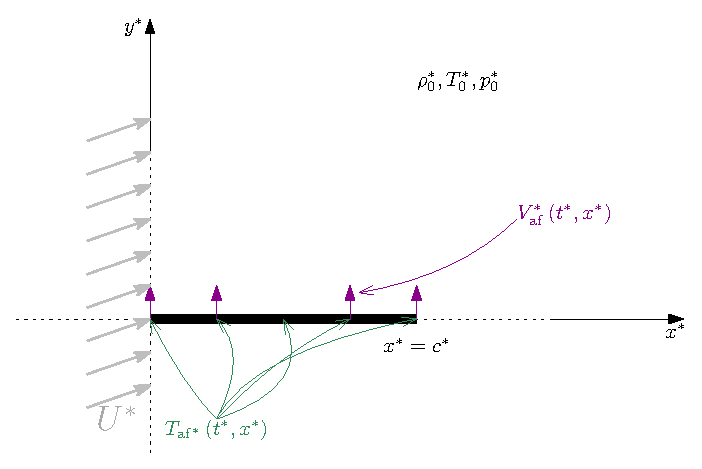
\includegraphics{drawings/problem_description.eps}
    \caption{\footnotesize Schematic of the Airfoil in a Uniform Flow: The drawing depicts an infinite gas layer confined by fully diffuse airfoil with length $c^*$, where the airfoil actuated by a prescribed small amplitude time and $x^*$-dependent normal velocity profile, and temperature profile denoted as $V_\af^*(t^*,x^*)$, $T_\af^*(t^*,x^*)$. The gas layer is subjected to a uniform flow denoted by $U^*$. The far field characteristics of the fluid, including density $\rho_0^*$, temperature $T_0^*$, and pressure $p_0^*$, are indicated.}
    \label{fig:problem_description}
\end{figure}
The airfoil-normal velocity amplitude, $v_\af$, is scaled by $\mathcal{U}_{\mathrm{th}}^*=\sqrt{2\mathcal{R}^*T_0^*}$, where $\mathcal{R}^*$ is the specific gas constant. The oscillations of the airfoil's temperature are also taken into consideration and are represented by a function of time and position along the $x^*$ axis
\begin{equation} \label{eq:T_af}
    T_\af^*=T_\af^*\left(t^*,x^*\right)
    .
\end{equation}

Since $\varepsilon\ll 1$, the airfoil is assumed to be staying on its initial position, merged with the abscissa. The airfoil is assumed to be fully diffuse, with both its temperature and velocity oscillating as a function of time. The solution of the problem in this research project aims to investigate the behavior of the gas layer under these conditions, taking into account the effects of small-amplitude time-harmonic oscillations.

The present study explores the impact of gas rarefaction on the propagation of hydrodynamic field changes generated by airfoil excitation in a two-dimensional setting. The changes are described by the airfoil's normal velocity, denoted as $V_\af^*(x^*,t^*)$, and temperature, denoted as $T_\af^*(x^*,t^*)$, which are functions of horizontal location and time. The degree of gas rarefaction is determined by the ratio of the time frequency of imposed oscillations, denoted as $\omega^*$, to the mean collision frequency of gas molecules, approximated as $v_0^*\approx \mathcal{U}_{\mathrm{th}}^* / \lambda^*$, where $\lambda^*$ represents the mean free path of gas molecules. Our focus is on investigating the regime of high rarefaction, known as the ballistic limit, which is expected to occur at large values of $\omega^* \lambda^* / \mathcal{U}_{\mathrm{th}}^*$. By using $\omega^{*-1}$ and $\mathcal{U}_{\mathrm{th}}^*$ as the characteristic time and velocity scales of the problem, respectively, the resulting length-scale is of the order of the acoustic wavelength, $\mathcal{U}_{\mathrm{th}}^* / \omega^*$. The governing parameter of the problem is the Knudsen number, defined as
\begin{equation} \label{eq:Knud}
 \Kn
 =
 \omega^* \lambda^* / \mathcal{U}_{\mathrm{th}}^*
 ,
\end{equation}
which represents the ratio of the characteristic length-scale to the mean free path, and the amplitude of $V_\af^*\left(x^*,t^*\right)$, which represents the prescribed airfoil vibration amplitude. To complete the non-dimensional description, we adopt $\rho_0^*$ and $T_0^*$ as the reference gas density and temperature, respectively, and normalize length dimensions by the length of the airfoil. In the subsequent analysis, we investigate the specific limits of highly rarefied conditions, expected at $\Kn \gg 1$, using analytical methods.

\section{Analytical Analysis}
Within the context of gas kinetic theory and a two-dimensional configuration, the gas state is described by the probability density function $f=f\left(t,x,y,\boldsymbol{\xi}\right)$, which represents the likelihood of finding a gas molecule with velocity $\boldsymbol{\xi}=\left(\xi_x,\xi_y,\xi_z\right)$ near a position $\left(x,y\right)$ at time $t$. Under the assumption of linearized conditions, we express $f(t,x,y,\boldsymbol{\xi})$ as
\begin{equation} \label{eq:perturbed_Maxwell}
    f\left(t,x,y,\boldsymbol{\xi}\right)
    =
    F\left[1+\phi\left(t,x,y,\boldsymbol{\xi}\right)\right],
\end{equation}
where $F=\pi^{-3/2}e^{-\left|\boldsymbol{\xi}-\mathbf{U}\right|^2}$ represents the non-dimensional Maxwellian equilibrium distribution, and $\phi\left(t,x,y,\boldsymbol{\xi}\right)$ denotes the probability perturbation function.

The dimensionless Boltzmann equation without external forces is typically used to describe the behavior of a dilute gas of particles, such as molecules or atoms, undergoing binary collisions in the absence of external influences. The vector form of this equation can be written as follows\cite{kogan1969rarefied}:
\begin{equation} \label{eq:dimensionless_Boltzmann_vectorForm}
    \St\frac{\partial f}{\partial t} +\boldsymbol{\xi}\frac{\partial f}{\partial \boldsymbol{\xi}}
    =
    \frac{1}{\Kn}\int \left(f\prime f_1\prime-ff_1\right)\mathbf{g b}d\mathbf{b} d\boldsymbol{\varepsilon} d\boldsymbol{\xi}
\end{equation}
The right-hand side of Eq. \ref{eq:dimensionless_Boltzmann_vectorForm} represents the effect of binary collisions between gas particles, which is described by the collisions integral. In other words, it accounts for the interactions between pairs of gas particles as they collide and exchange energy and momentum. The collisions integral is a mathematical term that characterizes a sum over probability of particles colliding and the resulting change in their velocities. The Strouhal number denoted by $\St$ is a dimensionless parameter used in fluid dynamics to characterize the behavior of periodic or oscillatory flow phenomena, such as vortex shedding behind an object in a flowing fluid. It is defined as the ratio of the characteristic frequency of the flow to the product of the characteristic length and the characteristic velocity of the flow. In some cases, a common approximation used in fluid dynamics is assuming that the Strouhal number is equal to one ($\St\approx 1$). This approximation is often used when the frequency of the flow is roughly comparable to the product of the characteristic length and velocity, meaning that the flow exhibits a characteristic time scale that is on the order of the time required for the fluid to travel the characteristic length at the characteristic velocity. In such cases, the Strouhal number of one is considered a good assumption because it suggests that the fluid is responding to the imposed motion in a resonant or efficient manner, leading to significant flow phenomena such as vortex shedding, wake formation, or other dynamic behaviors.

In the regime of large Knudsen number, we consider the collisionless two-dimensional unsteady Boltzmann equation for $\phi\left(t,x,y,\boldsymbol{\xi}\right)$:
\begin{equation} \label{eq:Boltzman}
    \frac{\partial\phi}{\partial t}
    +
    \xi_x\frac{\partial\phi}{\partial x}
    +
    \xi_y\frac{\partial\phi}{\partial y}
    =
    0
    .
\end{equation}
The free-molecular problem can be solved in closed-form for an arbitrary (small-amplitude) sources, $V_\af=V_\af\left(t,x\right)$, $T_\af=T_\af\left(t,x\right)$. Therefore, we consider a more general problem that does not deductively assume time-harmonic (airfoil velocity or temperature) oscillations. Eq. \ref{eq:Boltzman} is subject to a far-field decay condition, along with a fully diffuse boundary condition at the airfoil position. The latter takes the form
\begin{equation} \label{eq:boundary_condition}
    \phi\left(t,0\leq x\leq 1,0,\xi_y \gtrless 0 \right)
    =
    \rho_\af^\pm\left(t,x\right)
    ,
\end{equation}
where $\rho_\af^\pm\left(t,x\right)$ is yet to be determined. The solution for Eq. \ref{eq:Boltzman} subject to Eq. \ref{eq:boundary_condition} is
\begin{equation} \label{eq:phi}
    \phi\left(t,x,y,\boldsymbol{\xi}\right)
    =
    \begin{cases}
        \rho_\af^\pm & ,\quad\{ y \gtrless 0 \} \cap \{ \xi_y \gtrless 0 \} \cap \{ \frac{x-1}{y}\xi_y \leq \xi_x \leq \frac{x}{y}\xi_y \} \\        
        0            & ,\quad\text{else}

    \end{cases}
    .
\end{equation}
In order to determine the airfoil functions $\rho_\af^\pm\left(t,x\right)$  as mentioned in Eq. \ref{eq:phi}, an impermeability condition is imposed on the normal velocity component $v\left(t,x,y\right)$, utilizing Eq. \ref{eq:perturbed_Maxwell} as well. This condition is given by
\begin{equation} \label{eq:impermeability}
    v\left(t,x,0^\pm\right)
    =
    \frac{\pi^{-3/2}}{\rho\left(t,x,0^\pm\right)} \left[ \int\limits_{\xi_y\lessgtr0}\xi_y F d\boldsymbol{\xi}  
    +
    \frac{1}{T_\af^{3/2}\left(t,x\right)}
    \int\limits_{\xi_y\gtrless0}\xi_y\phi F d\boldsymbol{\xi}    
    \right]
    =
    V_\af\left(t,x\right)
    .
\end{equation}
First calculating $\rho\left(t,x,0^\pm\right)$ to find
\begin{equation} \label{eq:rho_0}
    \rho\left(t,x,0^\pm\right)
    =
    \frac{1\mp\erf U_y}{2}
    +
    \rho_\af^\pm\left(t,x\right)\frac{1\pm\erf\eta}{2}
    ,
\end{equation}
where

\begin{equation}
    \erf z
    =
    \frac{2}{\sqrt{\pi}} \int_{0}^{z}e^{-t^2}dt\,,
\end{equation}
and $\eta$ denoting the ratio
\begin{equation} \label{eq:eta}
    \eta
    =
    \frac{V_\af\left(t,x\right)}{\sqrt{T_\af\left(t,x\right)}}
\end{equation}
By substituting Eqs. \ref{eq:phi}, \ref{eq:rho_0} and \ref{eq:eta}, into Eq. \ref{eq:impermeability}, the expression for $\rho_\af^\pm\left(t,x\right)$ is found to be
\begin{equation} \label{eq:rho_af}
    \rho_\af^\pm\left(t,x\right)
    =
    e^{+\eta^2}
    \left[ \frac{ e^{-U_y^2} + U_y\sqrt{\pi} \left( \erf U_y \mp 1 \right) }{ \sqrt{T_\af \left(t,x\right)} } - \eta\sqrt{\pi} \left( \erf U_y \mp 1 \right) \right]
    ,
\end{equation}
which indicates the local dependence of the gas mass flux at the airfoil both on its instantaneous velocity and temperature. Once $\phi\left(t,x,y,\boldsymbol{\xi}\right)$ is in our hand, using Eq. \ref{eq:perturbed_Maxwell} yields $f(t,\mathbf{x},\boldsymbol{\xi})$.

For practical uses, we successfully obtained the distribution function $f(t,\mathbf{x},\boldsymbol{\xi})$ which describes the microscopic behavior of gas particles in a system. The distribution function $f$, plays a pivotal role in the kinetic theory of gases, providing a comprehensive description of the statistical behavior of gas molecules. However, for many applications, it is often sufficient to consider only macroscopic quantities, such as density, velocity, stress tensor, and energy flux, which can be obtained through experimental measurements as well. In cases where the mean free path of gas molecules is sufficiently small, a hydrodynamic description of the gas is feasible. Nevertheless, it should be noted that a hydrodynamic approach entails averaging the distribution function $f(t,\mathbf{x},\boldsymbol{\xi})$ over the molecular scale to obtain macroscopic properties of interest.

Notably, the number of gas molecules, denoted as $n(t,\mathbf{x})$, in a given unit volume can be determined by integrating the distribution function $f(t,\mathbf{x},\boldsymbol{\xi})$ over all possible molecular velocities $\boldsymbol{\xi}$\cite{kogan1969rarefied}
\begin{equation} \label{eq:macro_number_density}
    n\left(t,x,y\right)
    =
    \int f\left(t,x,y,\boldsymbol{\xi}\right)d \boldsymbol{\xi}
    .
\end{equation}
Similarly, the mean velocity of the molecules, $\mathbf{u}(t,\mathbf{x})$, and the stress tensor, $P_{ij}$, can be calculated by
\begin{align}
    \mathbf{u}\left(t,x,y\right) &= \frac{1}{n}\int \boldsymbol{\xi}f\left(t,x,y,\boldsymbol{\xi}\right) d\boldsymbol{\xi} \label{eq:macro_velocity} \\
    P_{ij}\left(t,x,y\right) &= m\int c_jc_i f\left(t,x,y,\boldsymbol{\xi}\right) d\boldsymbol{\xi} \label{eq:macro_stress}
    .
\end{align}
Where $\mathbf{c}$, the peculiar velocity, defined as $\mathbf{c}=\boldsymbol{\xi}-\mathbf{u}$.
Moreover, a quantity $P$, defined as $2/3$ times the sum of the diagonal components of the stress tensor, coincides with the conventional pressure in the hydrodynamic description of gases. Remarkably, this relationship can be expressed as
\begin{equation}
    P(t,x,y)=n(t,x,y)\cdot k\cdot T(t,x,y)
    ,
\end{equation}
where $n(t,x,y)$ (from Eq. \ref{eq:macro_number_density}) represents the number density of gas molecules, $k$ is the Boltzmann constant, and $T(t,x,y)$ denotes the temperature.